%!TEX encoding = UTF-8 Unicode
%!TEX root = ../lect-w08.tex

%%%

% \ifkompendium\else

% \Subsection{Bonus}

% \begin{Slide}{Grupper, antal medlemmar, bonus}
% \begin{multicols}{2}
% 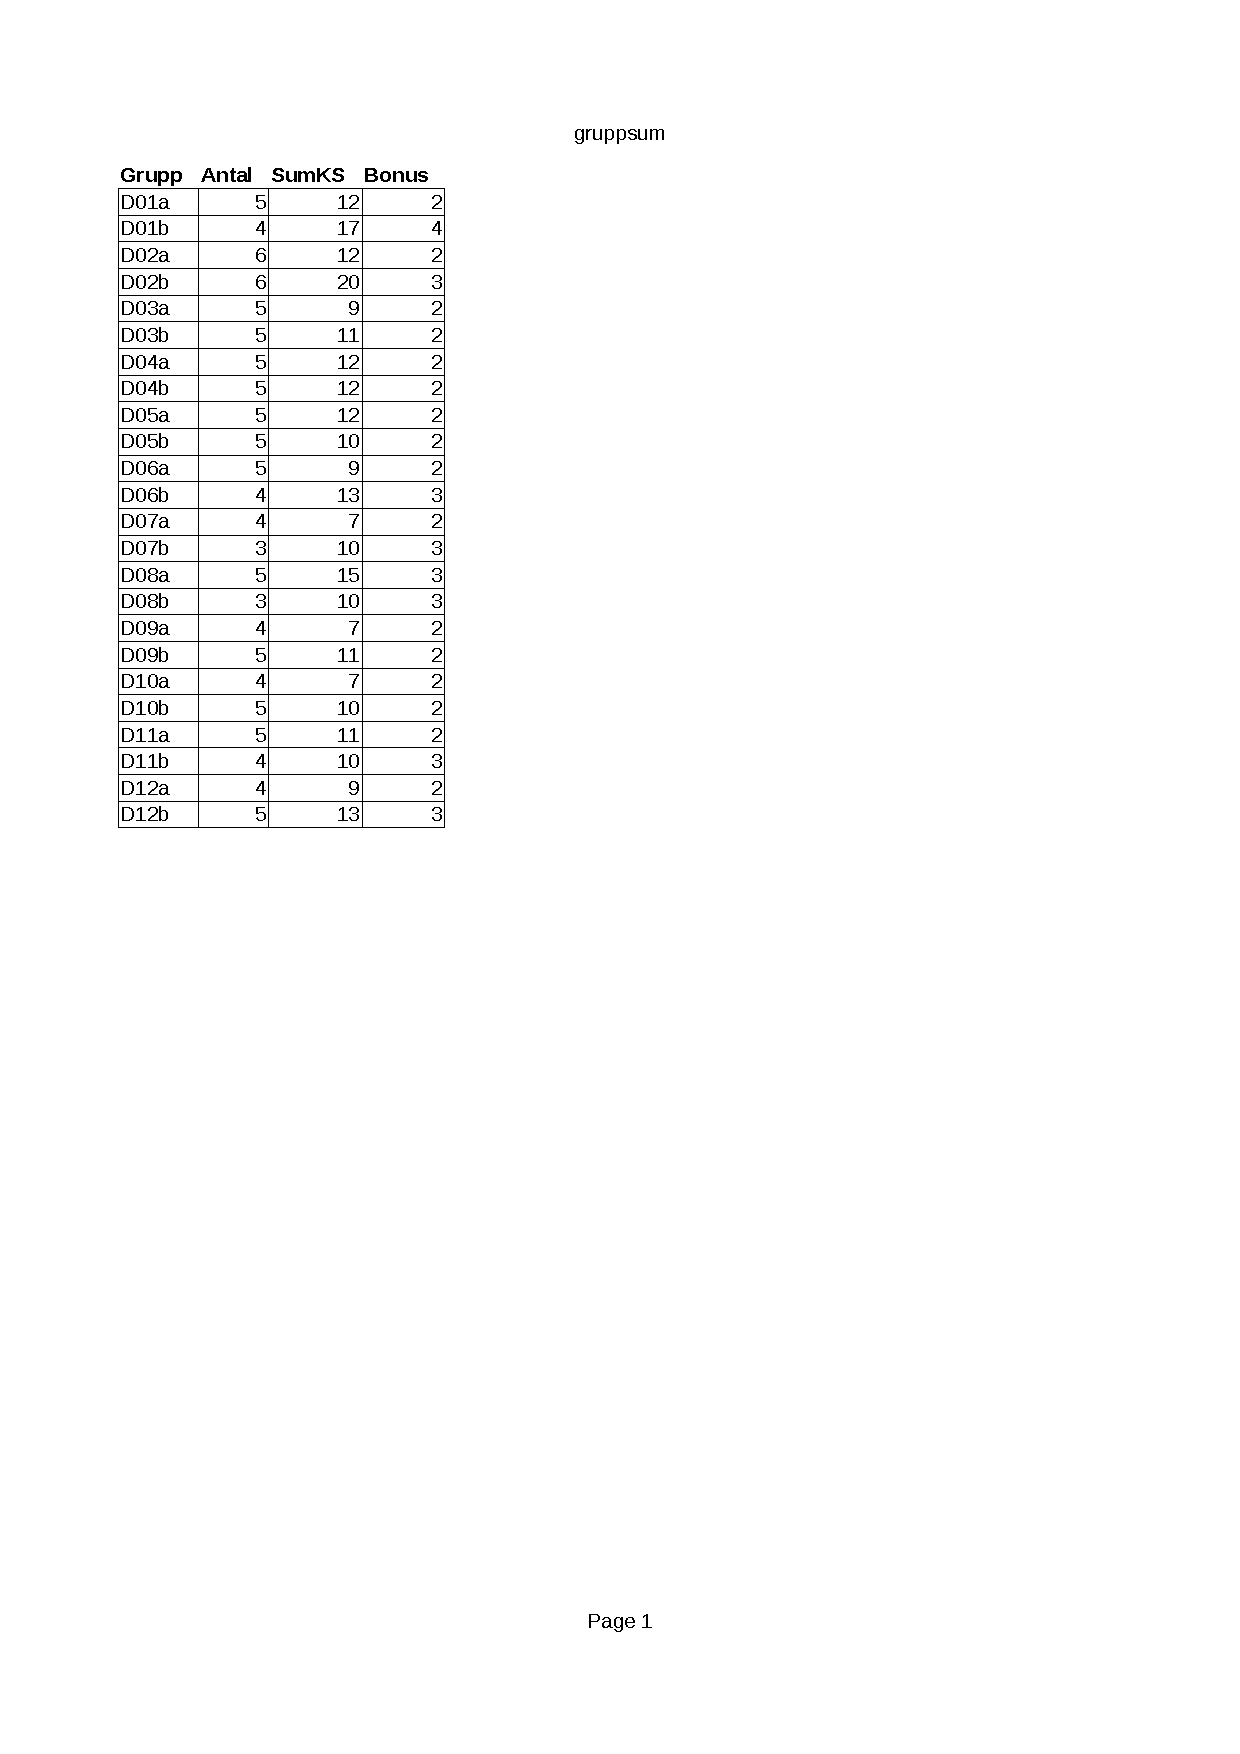
\includegraphics[clip, trim=0cm 1cm 3.2cm 2.5cm, width=0.9\textwidth]{../img/bonus-2016.pdf}

% \columnbreak

% \begin{itemize}
% \pause
% \item Bonus gäller vid första ordinarie tentatillfälle 
% \pause
% \item D07b och D08b har 3 st; \\ vill ni göra merge?

% \end{itemize}
% \end{multicols}
% \end{Slide}

% \Subsection{Specialundervisning}
% \begin{Slide}{Specialundervisning}
% Under vecka w09 och w10 (till att börja med) kommer vi att organisera \Emph{specialundervisning} under dessa \Alert{resurstider}:
% \begin{itemize}
% \item \Emph{Torsdag kl 8-10} i både \Alert{Falk} och \Alert{Val}  (Gustav, Valthor, Emil)
% \item \Emph{Torsdag kl 10-12} i \Alert{Falk} (Maj)
% \item OBS! Dessa rumtider är till för de som hade 0 eller 1 på kontrollskrivningen och som ansökt om specialundervisning via länk i speciell mejlinbjudan. 
% \end{itemize}
% \SlideFontSmall{Undantag: Om du har mer än 1 på kontrollskrivningen men inte alls har möjlighet att gå på någon annan resurstid än ovan är du också välkommen; anmäl då din situation till handledaren på plats och så får du vara med i gruppen och kan få svar på frågor etc. som vanligt.}
% \end{Slide}
% \fi











